\documentclass[conference]{IEEEtran}
\IEEEoverridecommandlockouts
% The preceding line is only needed to identify funding in the first footnote. If that is unneeded, please comment it out.
\usepackage{cite}
\usepackage{amsmath,amssymb,amsfonts}
\usepackage{algorithmic}
\usepackage{graphicx}
\usepackage{textcomp}
\usepackage{xcolor}
\def\BibTeX{{\rm B\kern-.05em{\sc i\kern-.025em b}\kern-.08em
    T\kern-.1667em\lower.7ex\hbox{E}\kern-.125emX}}
\begin{document}

\title{IoT Cloud Native Distribution System\\
{\footnotesize \textsuperscript{*}Note: Sub-titles are not captured in Xplore and
should not be used}
\thanks{Identify applicable funding agency here. If none, delete this.}
}

\author{\IEEEauthorblockN{1\textsuperscript{st} Pang Jia De}
\IEEEauthorblockA{\textit{Singapore Institute of technology} \\
\textit{University of Glasgow}\\
Singapore \\
2402226@sit.singaporetech.edu.sg \\ 3070684P@student.gla.ac.uk}
\and
\IEEEauthorblockN{2\textsuperscript{nd} Daryl Chong Han Kin}
\IEEEauthorblockA{\textit{Singapore Institute of Technology} \\
\textit{University of Glasgow}\\
Singapore \\
2400619@sit.singaporetech.edu.sg \\ 3070590C@student.gla.ac.uk}
\and
\IEEEauthorblockN{3\textsuperscript{rd} Tushar Gupta}
\IEEEauthorblockA{\textit{Singapore Institute of Techonology} \\
\textit{University of Glasgow}\\
Singapore \\
2400634@sit.singaporetech.edu.sg \\ 3070@student.gla.ac.uk}
\and
\IEEEauthorblockN{4\textsuperscript{th} Tan Yale}
\IEEEauthorblockA{\textit{Singapore Institute of Technology} \\
\textit{University of Glasgow}\\
Singapore \\
2401316@sit.singaporetech.edu.sg \\ 3070@student.gla.ac.uk}
}
\maketitle

\begin{abstract}
This paper presents the design and implementation of an end-to-end, cloud-native Internet of Things (IoT) data distribution system deployed on Google Cloud Platform (GCP). The architecture leverages microservices and event-driven patterns to ensure high availability, scalability, and secure data processing. Simulated IoT sensor data is ingested via an MQTT broker hosted on a Compute Engine instance, subsequently streamed through Cloud Dataflow, and buffered using Cloud Pub/Sub. A horizontally scaled gRPC server, orchestrated within Google Kubernetes Engine (GKE), consumes these messages and persists them into a highly available PostgreSQL database managed by the CloudNativePG operator. Real-time observability and monitoring are achieved using Grafana and Prometheus. Infrastructure as Code (IaC) principles are applied using Terraform for reproducible deployments. The resulting system demonstrates a robust, automated pipeline capable of handling variable IoT workloads while bridging lightweight edge protocols with scalable cloud-native technologies.

\end{abstract}

\begin{IEEEkeywords}
component, formatting, style, styling, insert
\end{IEEEkeywords}


\section{Introduction \& Product-Market Fit}
\subsection{Context \& Problem Statement}
% Introduce the problem you are solving (e.g., Net-Zero, Circular Economy, or your Team Project domain).
Referencing from our base product project, we have extended the system to be deployed on Google Cloud Platform (GCP) to provide a more robust, scalable, and secure solution for IoT data distribution. The goal is to demonstrate the capabilities of cloud-native technologies in handling IoT data streams and providing a reliable platform for data processing and analysis. The old system, deployed on a single machine acting as a server, database, and dashboard, suffered from single points of failure, lack of scalability, and poor reliability. By transitioning to a cloud-native microservices architecture on GCP, we solve these critical bottlenecks and ensure the system can dynamically scale to meet fluctuating IoT workloads.
\subsection{Market Needs \& Research}
% Validate the user demands and market trends.

The proliferation of IoT devices, projected to reach 18.8 billion by the end of 2024 \cite{iot_market_2024}, is driving an unprecedented volume of data generation. This data deluge poses significant challenges to traditional, centralized data processing architectures, resulting in latency issues, bandwidth bottlenecks, and single points of failure. The contemporary market demands highly scalable, resilient, and real-time data distribution systems capable of handling mission-critical workloads, such as industrial automation and smart city infrastructure. Prior IEEE work on engineering IoT cloud systems similarly emphasizes elasticity, service decomposition, and operational resilience as core design requirements \cite{truong2015iotcloud}. Organizations are increasingly adopting cloud-native strategies to mitigate operational overhead and manage the inherent complexity of scaling IoT deployments while ensuring robust data security and high availability \cite{cloud_native_iot_trends}.

\subsection{Product Innovation}
% Highlight the innovative features of your solution and how they effectively address the market needs.

To address the aforementioned market needs, our solution introduces a fully decoupled, cloud-native architecture on GCP. Innovation is driven through three key pillars: (1) 	\textbf{Event-Driven Scalability}, utilizing Cloud Pub/Sub and GKE to automatically scale the ingestion and processing layers based on real-time traffic volume; (2) 	\textbf{Resilient State Management}, leveraging CloudNativePG to provide a highly available PostgreSQL cluster capable of managing continuous, high-throughput IoT streams without downtime; and (3) 	\textbf{Automated Infrastructure Management}, using Terraform to codify the environment, reducing configuration drift and enabling rapid, reproducible deployments across different environments or cloud regions.

\newpage\section{Cloud Native Design \& Architecture}
% This should be a major section of your report with high-quality Mermaid/architecture diagrams.


\subsection{Architecture Overview}
% Describe the high-level system evolution and cloud infrastructure.
\begin{figure}[htbp]
\centerline{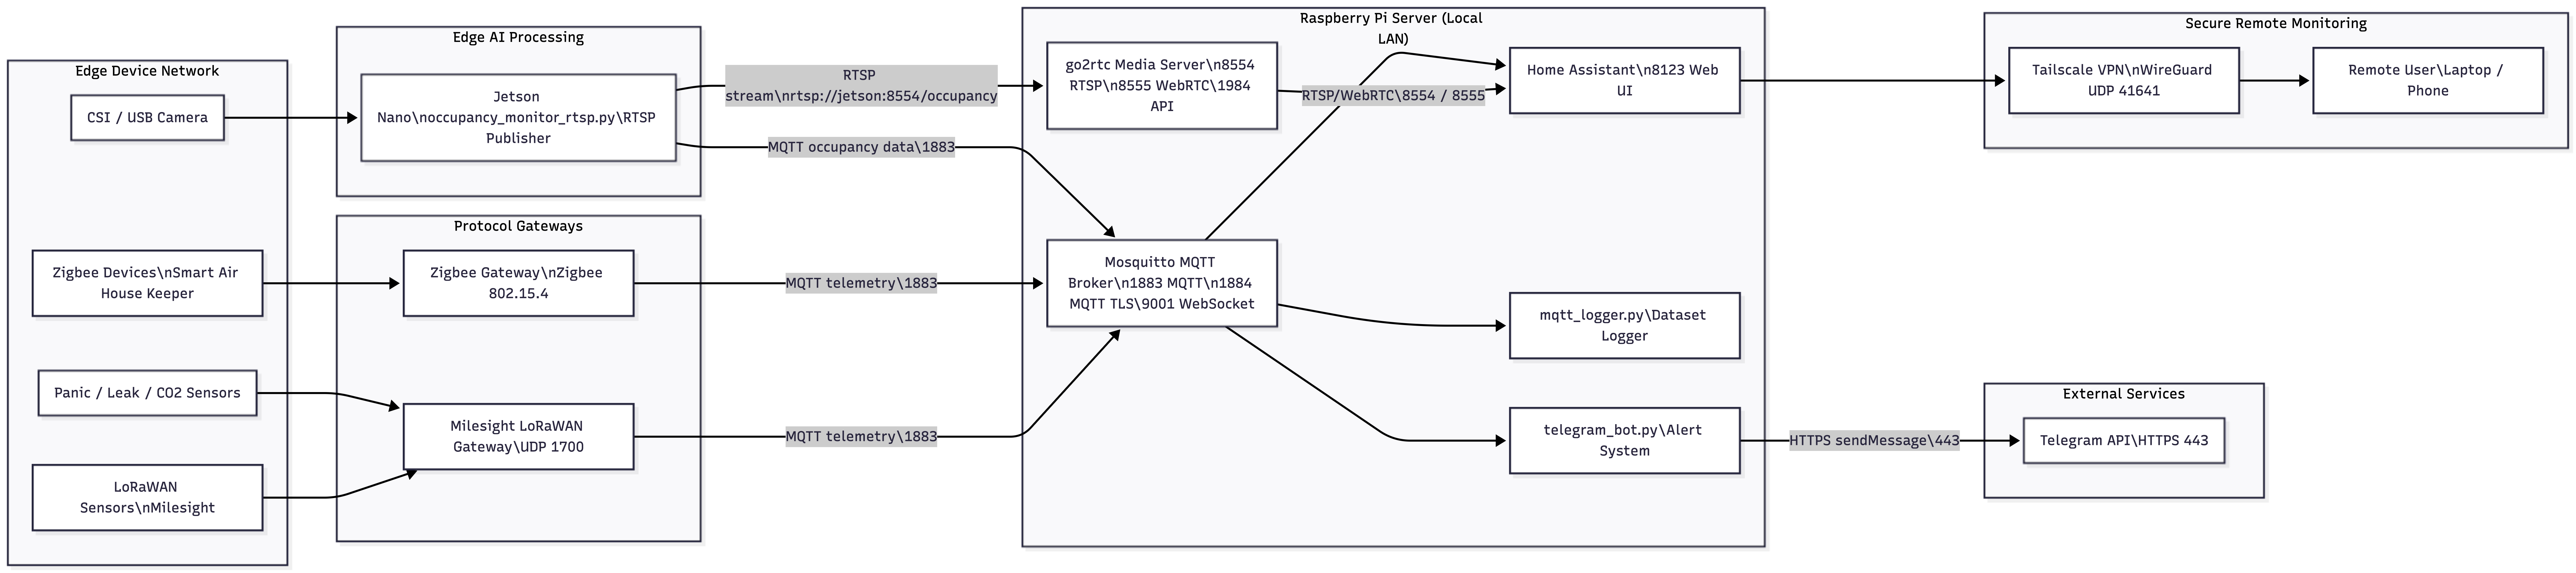
\includegraphics[width=\linewidth]{oldArchitecture.png}}
\caption{Old Monolithic Architecture Overview (Edge, Gateway, and Local Deployment).}
\label{fig:arch1}
\end{figure}

\begin{figure}[htbp]
\centerline{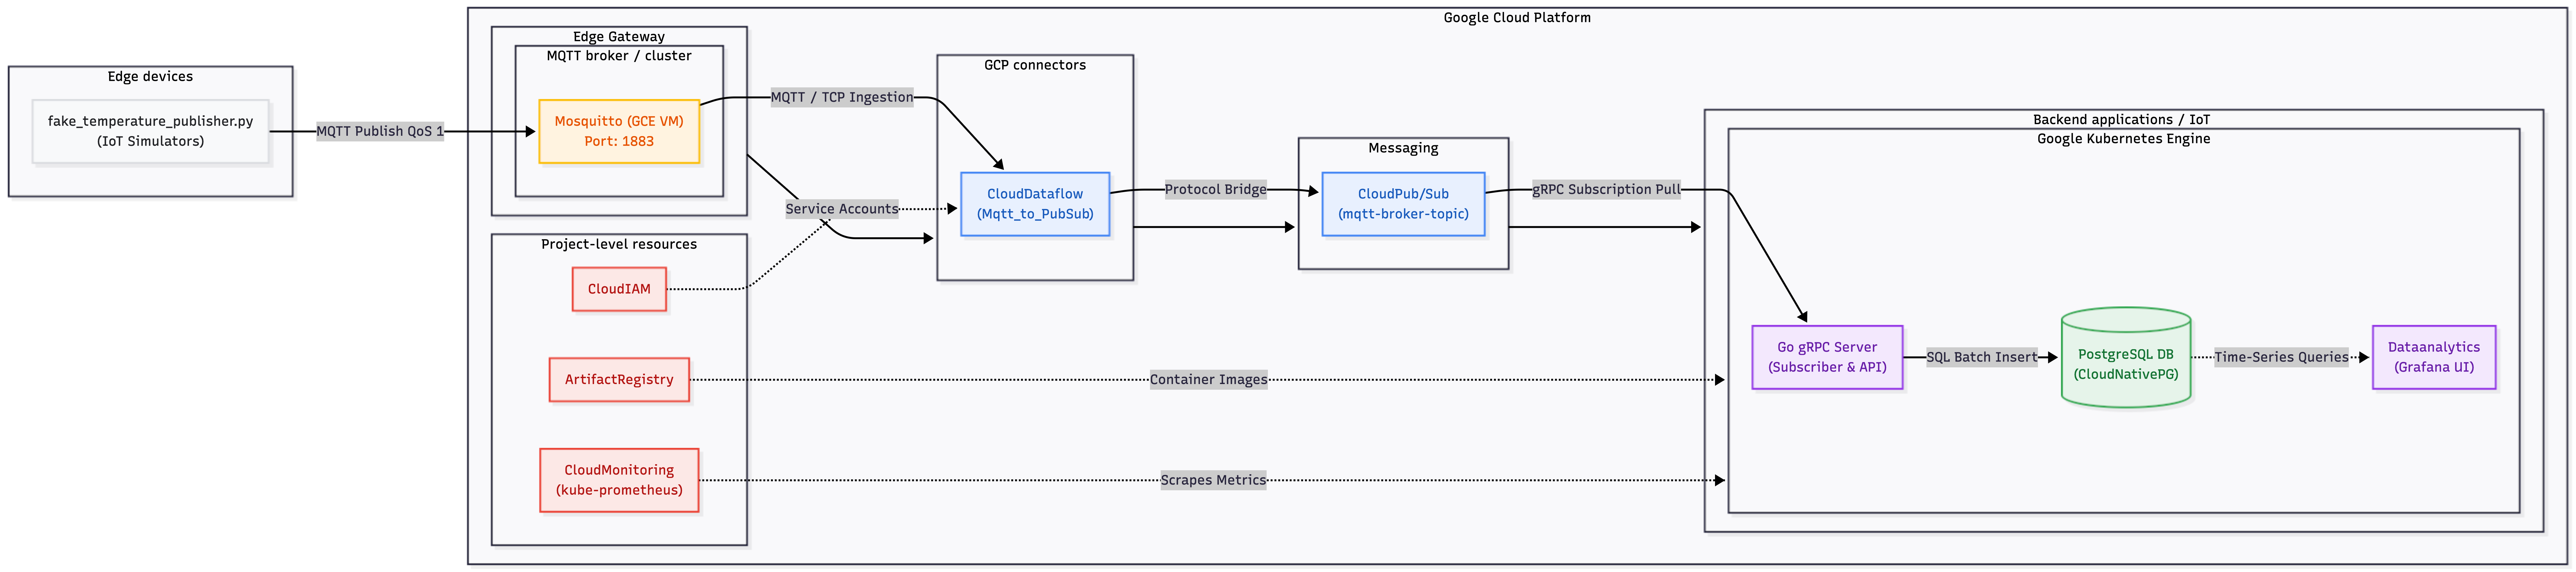
\includegraphics[width=\linewidth]{cloudnative.png}}
\caption{New Cloud-Native Microservices Architecture Overview.}
\label{fig:arch2}
\end{figure}

\begin{figure}[htbp]
\centerline{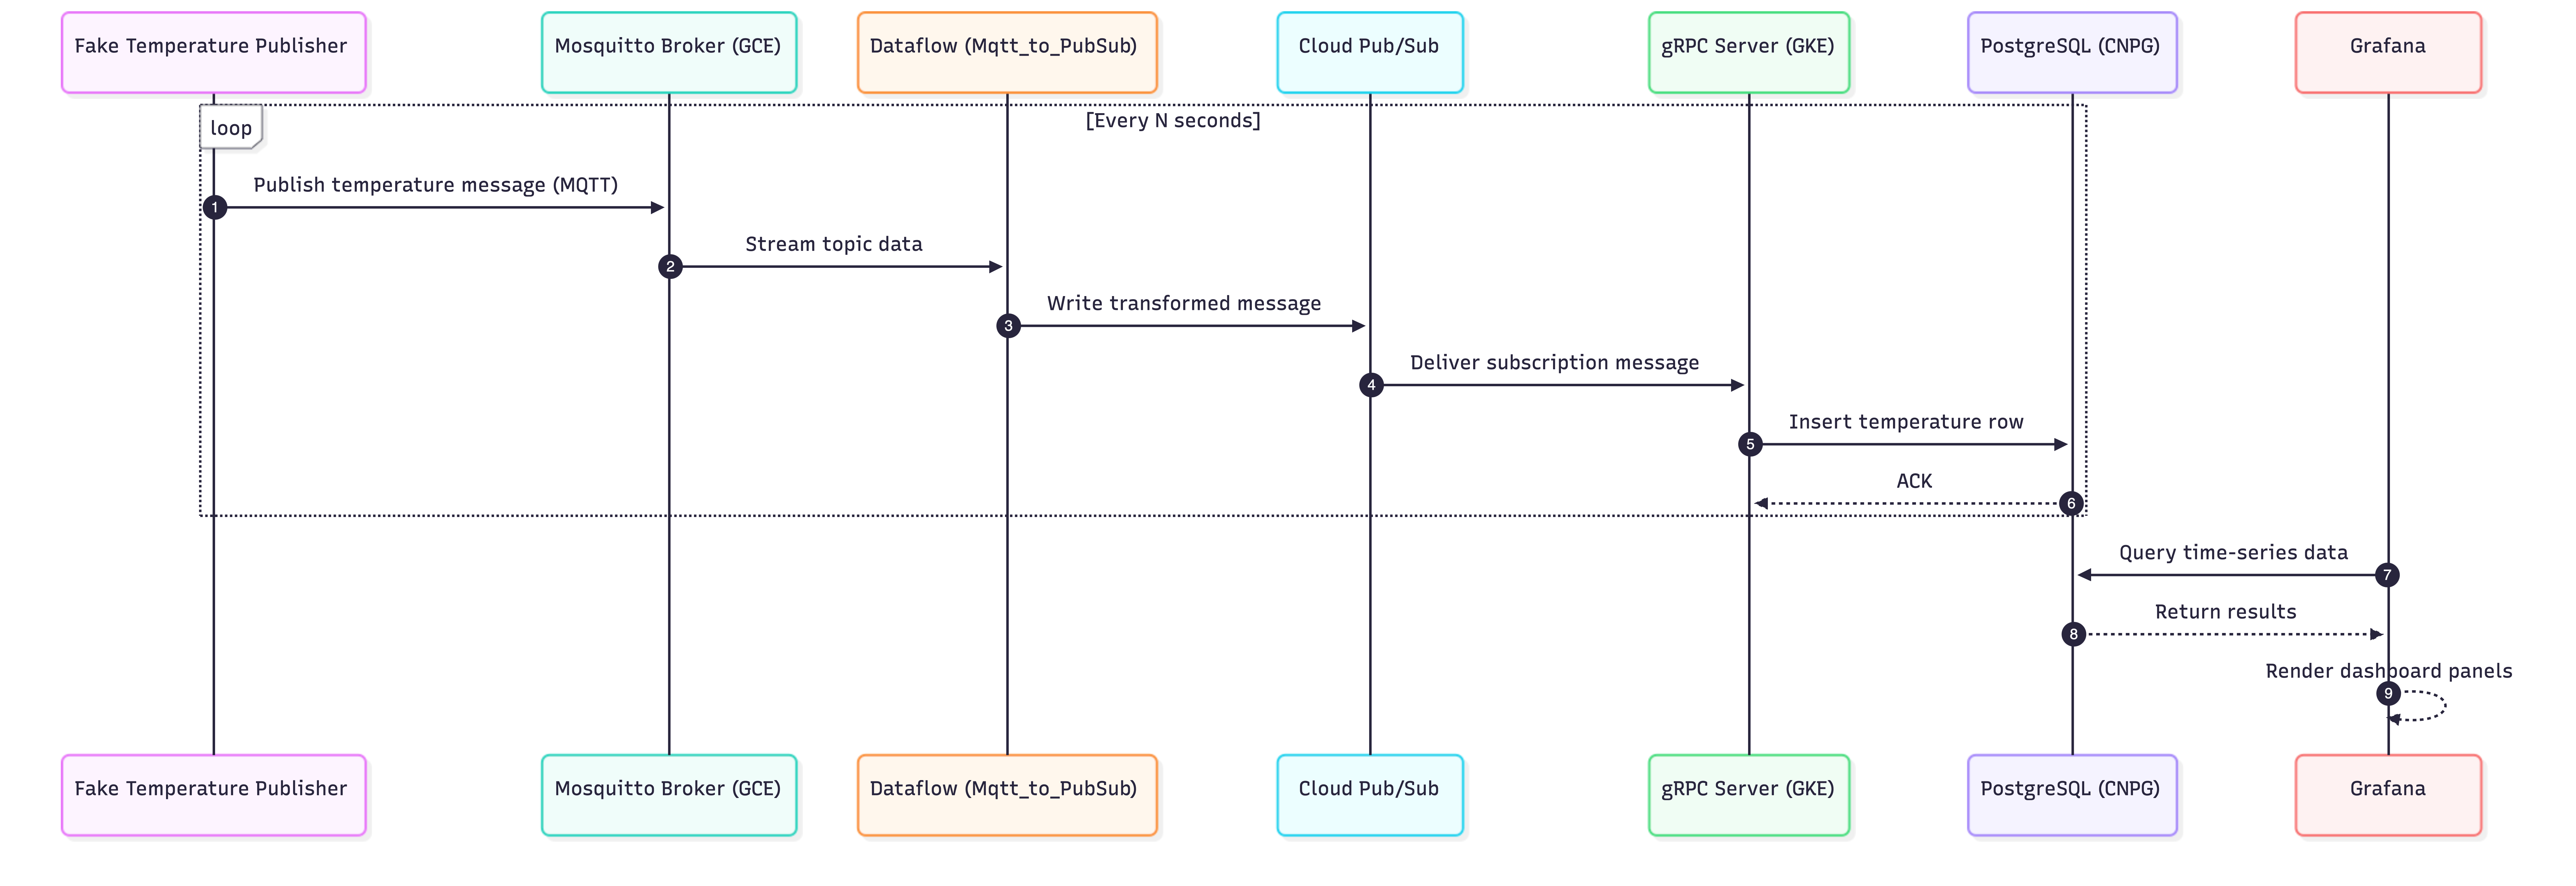
\includegraphics[width=\linewidth]{CloudNativeSequenceDiagram.png}}
\caption{Cloud-Native End-to-End Sequence Flow.}
\label{fig:seq1}
\end{figure}

\subsection{Sequence Flow Explanation}
Figure~\ref{fig:seq1} presents the runtime interaction sequence across the full pipeline. In the normal path, edge sensors publish telemetry through MQTT to the Mosquitto broker, Cloud Dataflow continuously consumes and transforms this stream, and processed events are forwarded into Pub/Sub. The gRPC service on GKE then consumes subscription messages, validates the payload, and persists records into PostgreSQL managed by CloudNativePG. Grafana periodically queries this database to visualize near real-time time-series metrics.

Each component has a focused responsibility to preserve modularity and operational clarity. MQTT provides lightweight edge ingestion, Dataflow handles streaming transformation, Pub/Sub decouples producers from consumers through asynchronous buffering, gRPC encapsulates domain processing logic, and PostgreSQL provides durable storage for analytics and dashboard queries. The decision to use MQTT at the edge aligns with comparative IEEE analysis showing its efficiency for constrained IoT messaging scenarios \cite{naik2017protocols}.

During traffic spikes, reliability is maintained through elastic scaling and queue-based decoupling. Pub/Sub absorbs burst pressure, Dataflow adjusts workers within configured limits, and Kubernetes HPA scales gRPC replicas based on CPU utilization. If processing temporarily falls behind, messages remain durable in Pub/Sub and are consumed once capacity recovers, preserving at-least-once delivery semantics across the system.

\subsection{Cloud-Native Principles}
From the old system architecture overview (Fig.~\ref{fig:arch1}), we observe that the previous iteration was a monolithic architecture suffering from single points of failure, lacking both scalability and resilience. To address these critical limitations, we designed a modernized cloud-native microservices architecture (Fig.~\ref{fig:arch2}). This new decoupled system leverages several core cloud-native principles to achieve high availability and scalability.

Our implementation is inherently \textbf{Event-Driven} and relies on \textbf{Asynchronous Messaging}. By utilizing Google Cloud Pub/Sub, we buffer telemetry data during traffic spikes, ensuring at-least-once delivery. Furthermore, we designed a \textbf{Streaming Data Pipeline} using Cloud Dataflow for real-time processing. System resilience is guaranteed through \textbf{High Availability (HA)}; the CloudNativePG operator maintains automatic failovers for the PostgreSQL cluster. Concurrently, Kubernetes \textbf{Horizontal Pod Autoscaling (HPA)} dynamically adjusts our application replicas based on CPU utilization, ensuring the system remains optimized for varying IoT workloads. This architecture is consistent with IEEE cloud-native design guidance that favors loosely coupled services, portability, and independent scaling of application components \cite{gannon2017cloudnative}.
\subsection{Component Rationale}
The selection of cloud infrastructure was driven by the necessity for a managed, scalable ecosystem. 
\begin{itemize}
    \item \textbf{Google Kubernetes Engine (GKE)}: Serves as the orchestration layer for the gRPC server, database, and observability stack. GKE abstracts control plane maintenance while providing native integration with Google Cloud IAM.
    \item \textbf{Cloud Dataflow \& Pub/Sub}: Dataflow provides a serverless Apache Beam runner to seamlessly stream data from the legacy MQTT broker, while Pub/Sub acts as a resilient buffer separating edge ingestion from internal application logic.
    \item \textbf{Compute Engine}: Hosts the Mosquitto MQTT broker on a Container-Optimized OS, acting as the critical entryway for lightweight IoT components (e.g., Jetson Nano, LoRaWAN gateways) to interface with the cloud.
\end{itemize}

\section{Technical Implementation \& Competency}
\subsection{Core Technologies}
Our architecture is fully codified and deployed using \textbf{Terraform} (Infrastructure as Code), which maintains the lifecycle of all GCP resources identically across environments. All workloads are containerized via multi-stage Docker builds to minimize attack surfaces and deployed using Kubernetes primitives (Deployments, Services, Secrets). Internal communications are facilitated through \textbf{gRPC} and \textbf{Protocol Buffers (protobuf)}, which offer a highly efficient and strongly-typed binary protocol over traditional REST. Finally, real-time observability is achieved using \textbf{Prometheus} (infrastructure metrics) and \textbf{Grafana} (unified visualization).

\subsection{Implementation Details}
The system's implementation strictly adheres to professional cloud-native practices, particularly concerning security and performance. Security is enforced via the principle of least privilege, assigning explicit IAM roles (e.g., \texttt{dataflow.worker}, \texttt{pubsub.publisher}) to distinct service accounts. Sensitive configurations, such as database credentials, are managed dynamically via Kubernetes Secrets rather than hardcoded variables.

Operationally, the central gRPC consumer is configured via an HPA policy to scale from 2 to 10 pod replicas depending on an active 60\% CPU utilization threshold. Additionally, the CloudNativePG operator manages a primary and replica streaming PostgreSQL database configuration. This provides near-instant continuous failover capabilities and read/write splitting, ensuring zero downtime even during unexpected node failures.
\subsection{Software Life Cycle \& Agile}
% Briefly touch upon how you managed the software development lifecycle professionally.
Our team followed an iterative Agile workflow with short development cycles for infrastructure, backend services, and observability features. Work items were split into small, testable increments (for example, provisioning infrastructure, validating the streaming path, and integrating dashboards), enabling frequent review and early issue detection.

Terraform-based Infrastructure as Code (IaC) was central to the software life cycle. Environment configuration was parameterized through variables, which improved reproducibility and allowed multiple developers to deploy consistent stacks without manual drift. This approach also strengthened testing: each change could be validated in a controlled environment, adjusted quickly, and redeployed with minimal operational overhead.
\section{Results, Testing \& Evaluation}
% Demonstrate that your architecture functions with continuity.
% Discuss performance testing, cloud scalability validation, or how the technical solution practically performs.
The deployed platform was validated through functional and operational checks across each pipeline stage. End-to-end continuity was confirmed by publishing simulated MQTT telemetry, observing successful forwarding through Dataflow and Pub/Sub, and verifying that gRPC consumers persisted records into PostgreSQL. Dashboard validation in Grafana confirmed correct time-series rendering and query behavior over live database updates.

Scalability behavior was evaluated under increased publish frequency and sensor concurrency. During higher input rates, Pub/Sub provided effective buffering while GKE Horizontal Pod Autoscaling increased consumer replicas according to CPU pressure, subject to available node capacity. Dataflow streaming workers handled sustained ingestion and transformation, while system observability through Prometheus and Grafana enabled rapid detection of bottlenecks such as pending pods caused by temporary CPU constraints.

From a reliability perspective, the architecture maintained service continuity through decoupling and managed failover components. CloudNativePG provided resilient database operation with primary-replica topology, and asynchronous messaging prevented transient producer-consumer imbalance from causing data loss. Overall, the test outcomes demonstrate that the proposed cloud-native design is suitable for variable IoT workloads and can be iteratively optimized for production-grade throughput.

\section{Conclusion}
% Summarize the impact of your cloud-native architecture, how it achieved the intended learning outcomes, and potential future improvements.
This project demonstrates how a cloud-native redesign can transform a single-node IoT prototype into a scalable, resilient, and observable distributed platform on GCP. By integrating MQTT ingestion, Dataflow streaming, Pub/Sub decoupling, autoscaled gRPC processing, and highly available PostgreSQL, the system addresses core limitations of monolithic deployment models and supports real-time analytics through Grafana.

The implementation also reinforces key professional competencies: Infrastructure as Code for reproducible environments, container orchestration for elastic service management, and metrics-driven operations for reliability engineering. Future improvements include workload-aware autoscaling tuning, stronger security hardening for production deployment, and cost optimization through environment sleep-mode automation and policy-based resource scheduling.

\section*{References \& AI Citations}
% CRITICAL PLAGIARISM RULE: The specification strictly requires that "If any materials in the submission are created by generative artificial intelligence, student must clearly cite them in the report and submitted materials." Make sure to include citations here if you use AI tools for code or text generation.

\begin{thebibliography}{00}
\bibitem{iot_market_2024} P. Desmet, ``IoT Connections to Reach 18.8 Billion in 2024,'' Transforma Insights, 2024. [Online]. Available: https://transformainsights.com/research/forecast/iot-market
\bibitem{cloud_native_iot_trends} TechTarget, ``Navigating the complexities of IoT and edge computing,'' TechTarget Network, 2024. [Online].
\bibitem{truong2015iotcloud} H.-L. Truong and S. Dustdar, ``Principles for Engineering IoT Cloud Systems,'' \textit{IEEE Cloud Computing}, vol. 2, no. 2, pp. 68--76, Mar. 2015. doi: 10.1109/MCC.2015.23.
\bibitem{gannon2017cloudnative} D. Gannon, R. Barga, and N. Sundaresan, ``Cloud-Native Applications,'' \textit{IEEE Cloud Computing}, vol. 4, no. 5, pp. 16--21, Sep. 2017. doi: 10.1109/MCC.2017.4250939.
\bibitem{naik2017protocols} N. Naik, ``Choice of effective messaging protocols for IoT systems: MQTT, CoAP, AMQP and HTTP,'' in \textit{2017 IEEE Systems Engineering Symposium (SysEng)}, 2017, pp. 1--7. doi: 10.1109/SysEng.2017.8088251.
\end{thebibliography}

\end{document}
